The DPC++ library consists of the following components:\par

\begin{itemize}
	\item A set of tested C++ standard APIs—we simply need to include the corresponding C++ standard header files and use the std namespace.
	\item Parallel STL that includes corresponding header files. We simply use \#include <dpstd/...> to include them. The DPC++ library uses namespace dpstd for the extended API classes and functions.
\end{itemize}

\hspace*{\fill} \par %插入空行
\textbf{Standard C++ APIs in DPC++}

The DPC++ library contains a set of tested standard C++ APIs. The basic functionality for a number of C++ standard APIs has been developed so that these APIs can be employed in device kernels similar to how they are employed in code for a typical C++ host application. Figure 18-7 shows an example of how to use std::swap in device code.\par

\hspace*{\fill} \par %插入空行
Figure 18-7. Using std::swap in device code
\begin{lstlisting}[caption={}]
class KernelSwap;
std::array <int,2> arr{8,9};
buffer<int> buf{arr};

{
	host_accessor host_A(buf);
	std::cout << "Before: " << host_A[0] << ", " << host_A[1] << "\n";
} // End scope of host_A so that upcoming kernel can operate on buf

queue Q;
Q.submit([&](handler &h) {
	accessor A{buf, h};
	h.single_task([=]() {
		// Call std::swap!
		std::swap(A[0], A[1]);
	});
});

host_accessor host_B(buf);
std::cout << "After: " << host_B[0] << ", " << host_B[1] << "\n";
\end{lstlisting}

We can use the following command to build and run the program (assuming it resides in the stdswap.cpp file):\par

\begin{tcolorbox}[colback=white,colframe=black]
dpcpp –std=c++17 stdswap.cpp –o stdswap.exe ./stdswap.exe
\end{tcolorbox}

The printed result is:\par

\begin{tcolorbox}[colback=white,colframe=black]
8, 9\\
9, 8
\end{tcolorbox}

Figure 18-8 lists C++ standard APIs with “Y” to indicate those that have been tested for use in DPC++ kernels for CPU, GPU, and FPGA devices, at the time of this writing. A blank indicates incomplete coverage (not all three device types) at the time of publication for this book. A table is also included as part of the online DPC++ language reference guide and will be updated over time—the library support in DPC++ will continue to expand its support.\par

In the DPC++ library, some C++ std functions are implemented based on their corresponding built-in functions on the device to achieve the same level of performance as the SYCL versions of these functions.\par

\hspace*{\fill} \par %插入空行
Figure 18-8. Library support with CPU/GPU/FPGA coverage (at time of book publication)
\begin{center}
	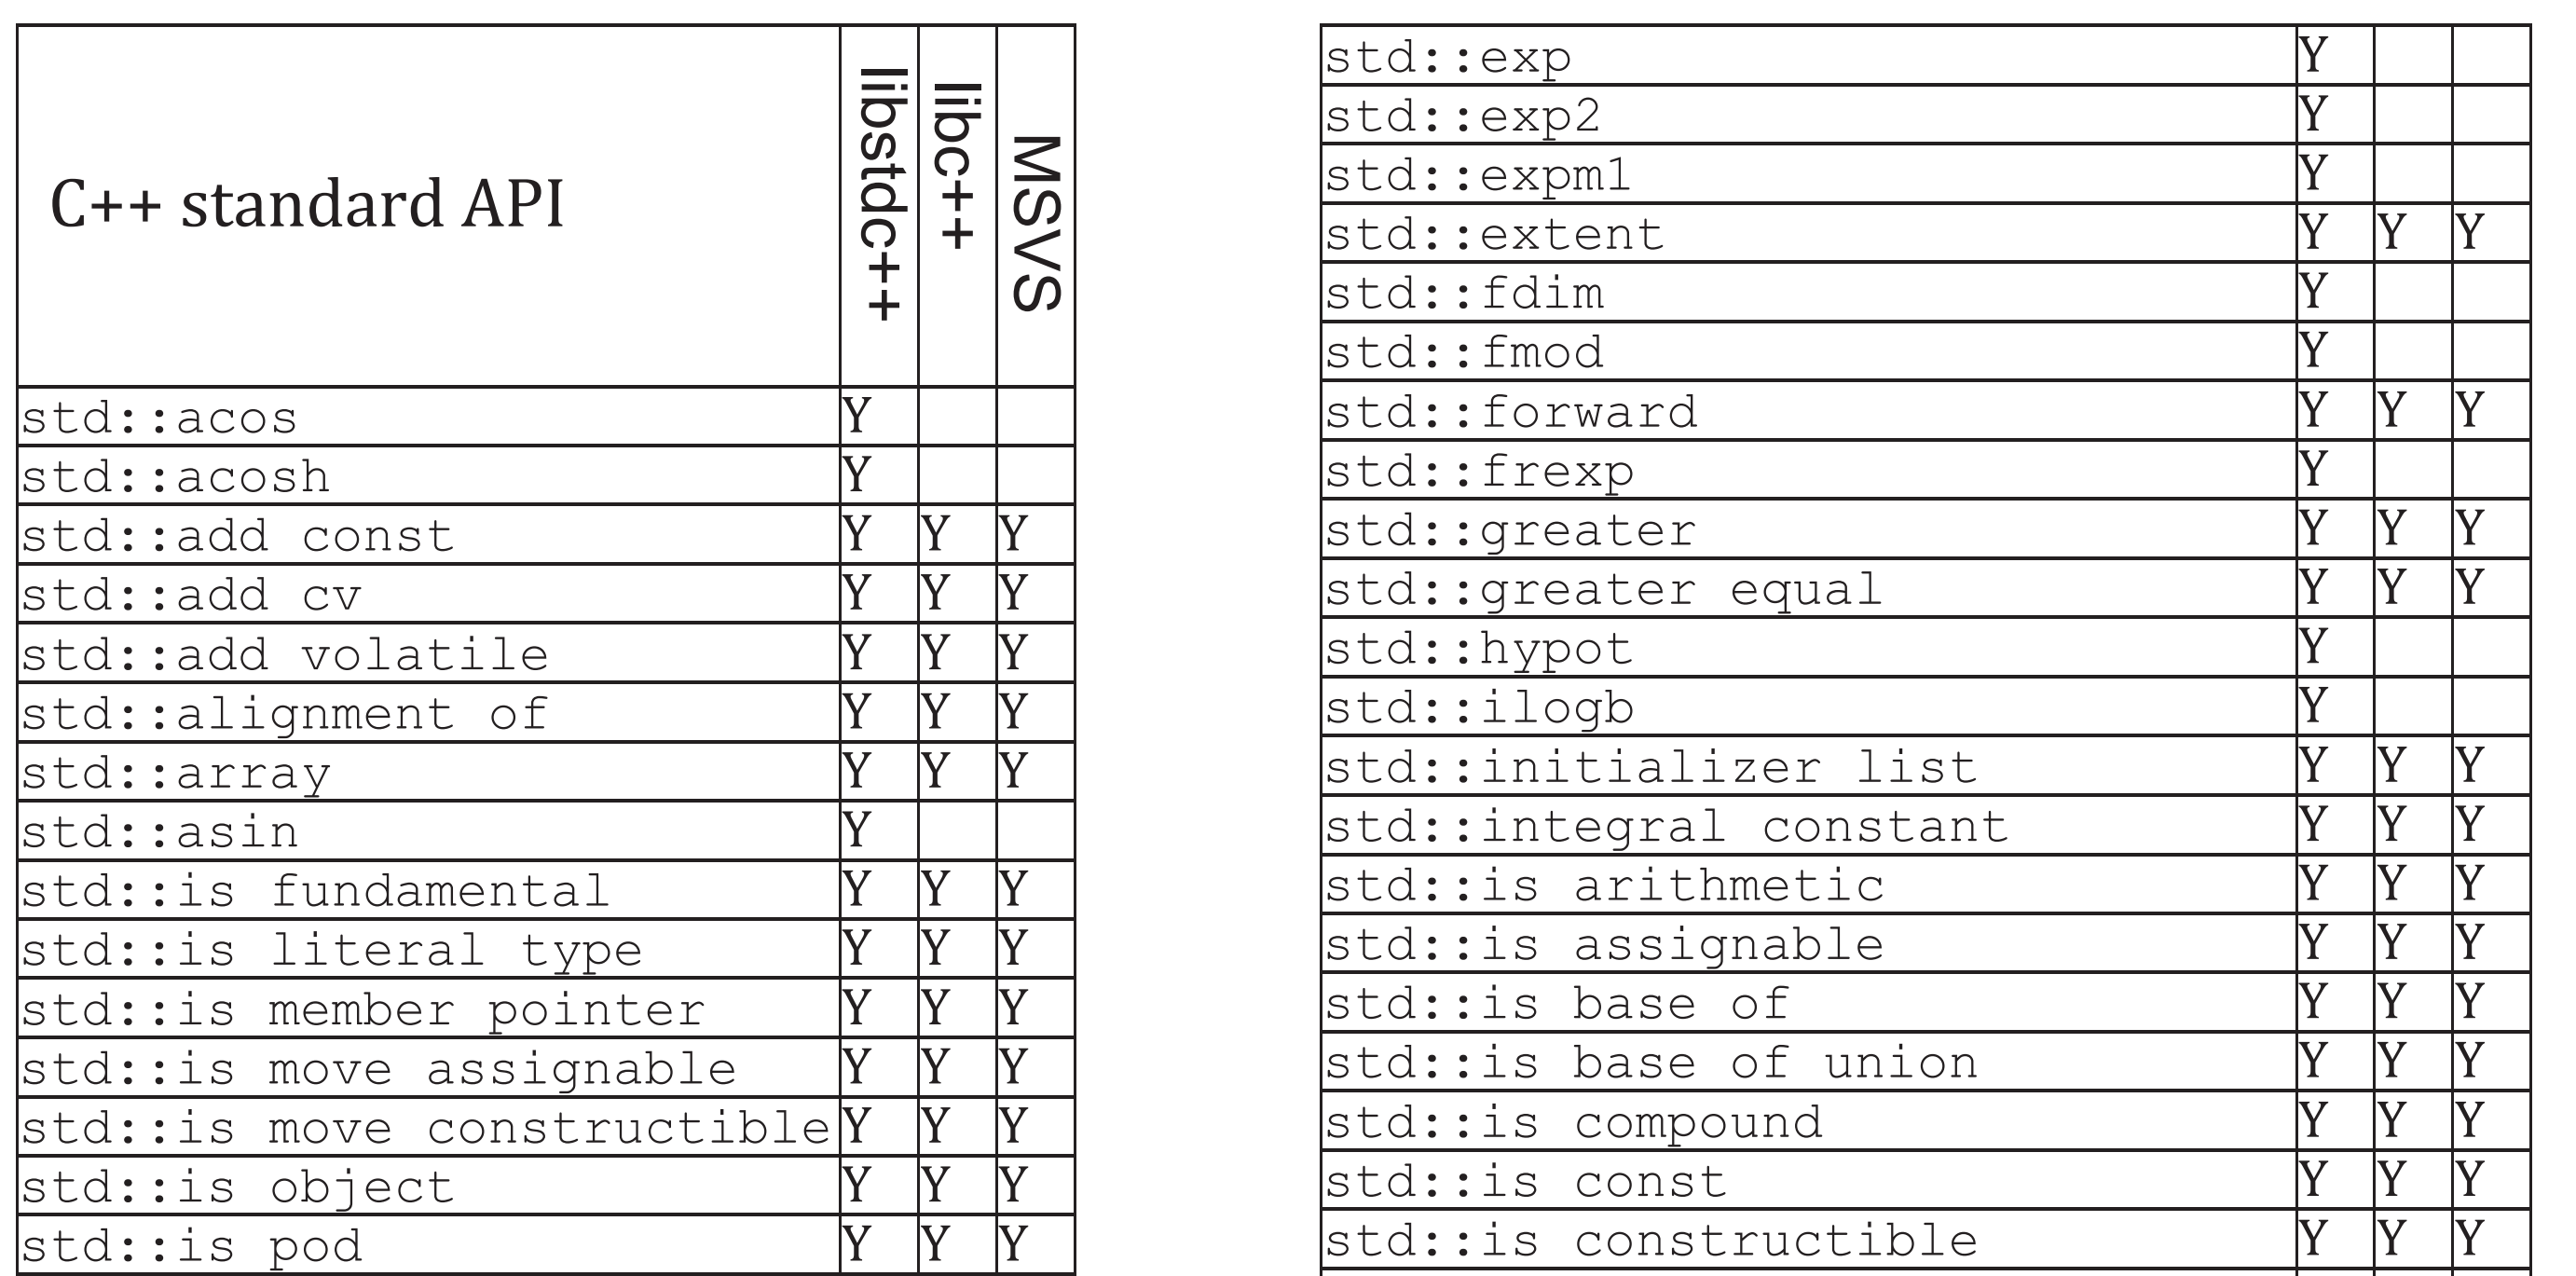
\includegraphics[width=1.0\textwidth]{content/chapter-18/images/7}
	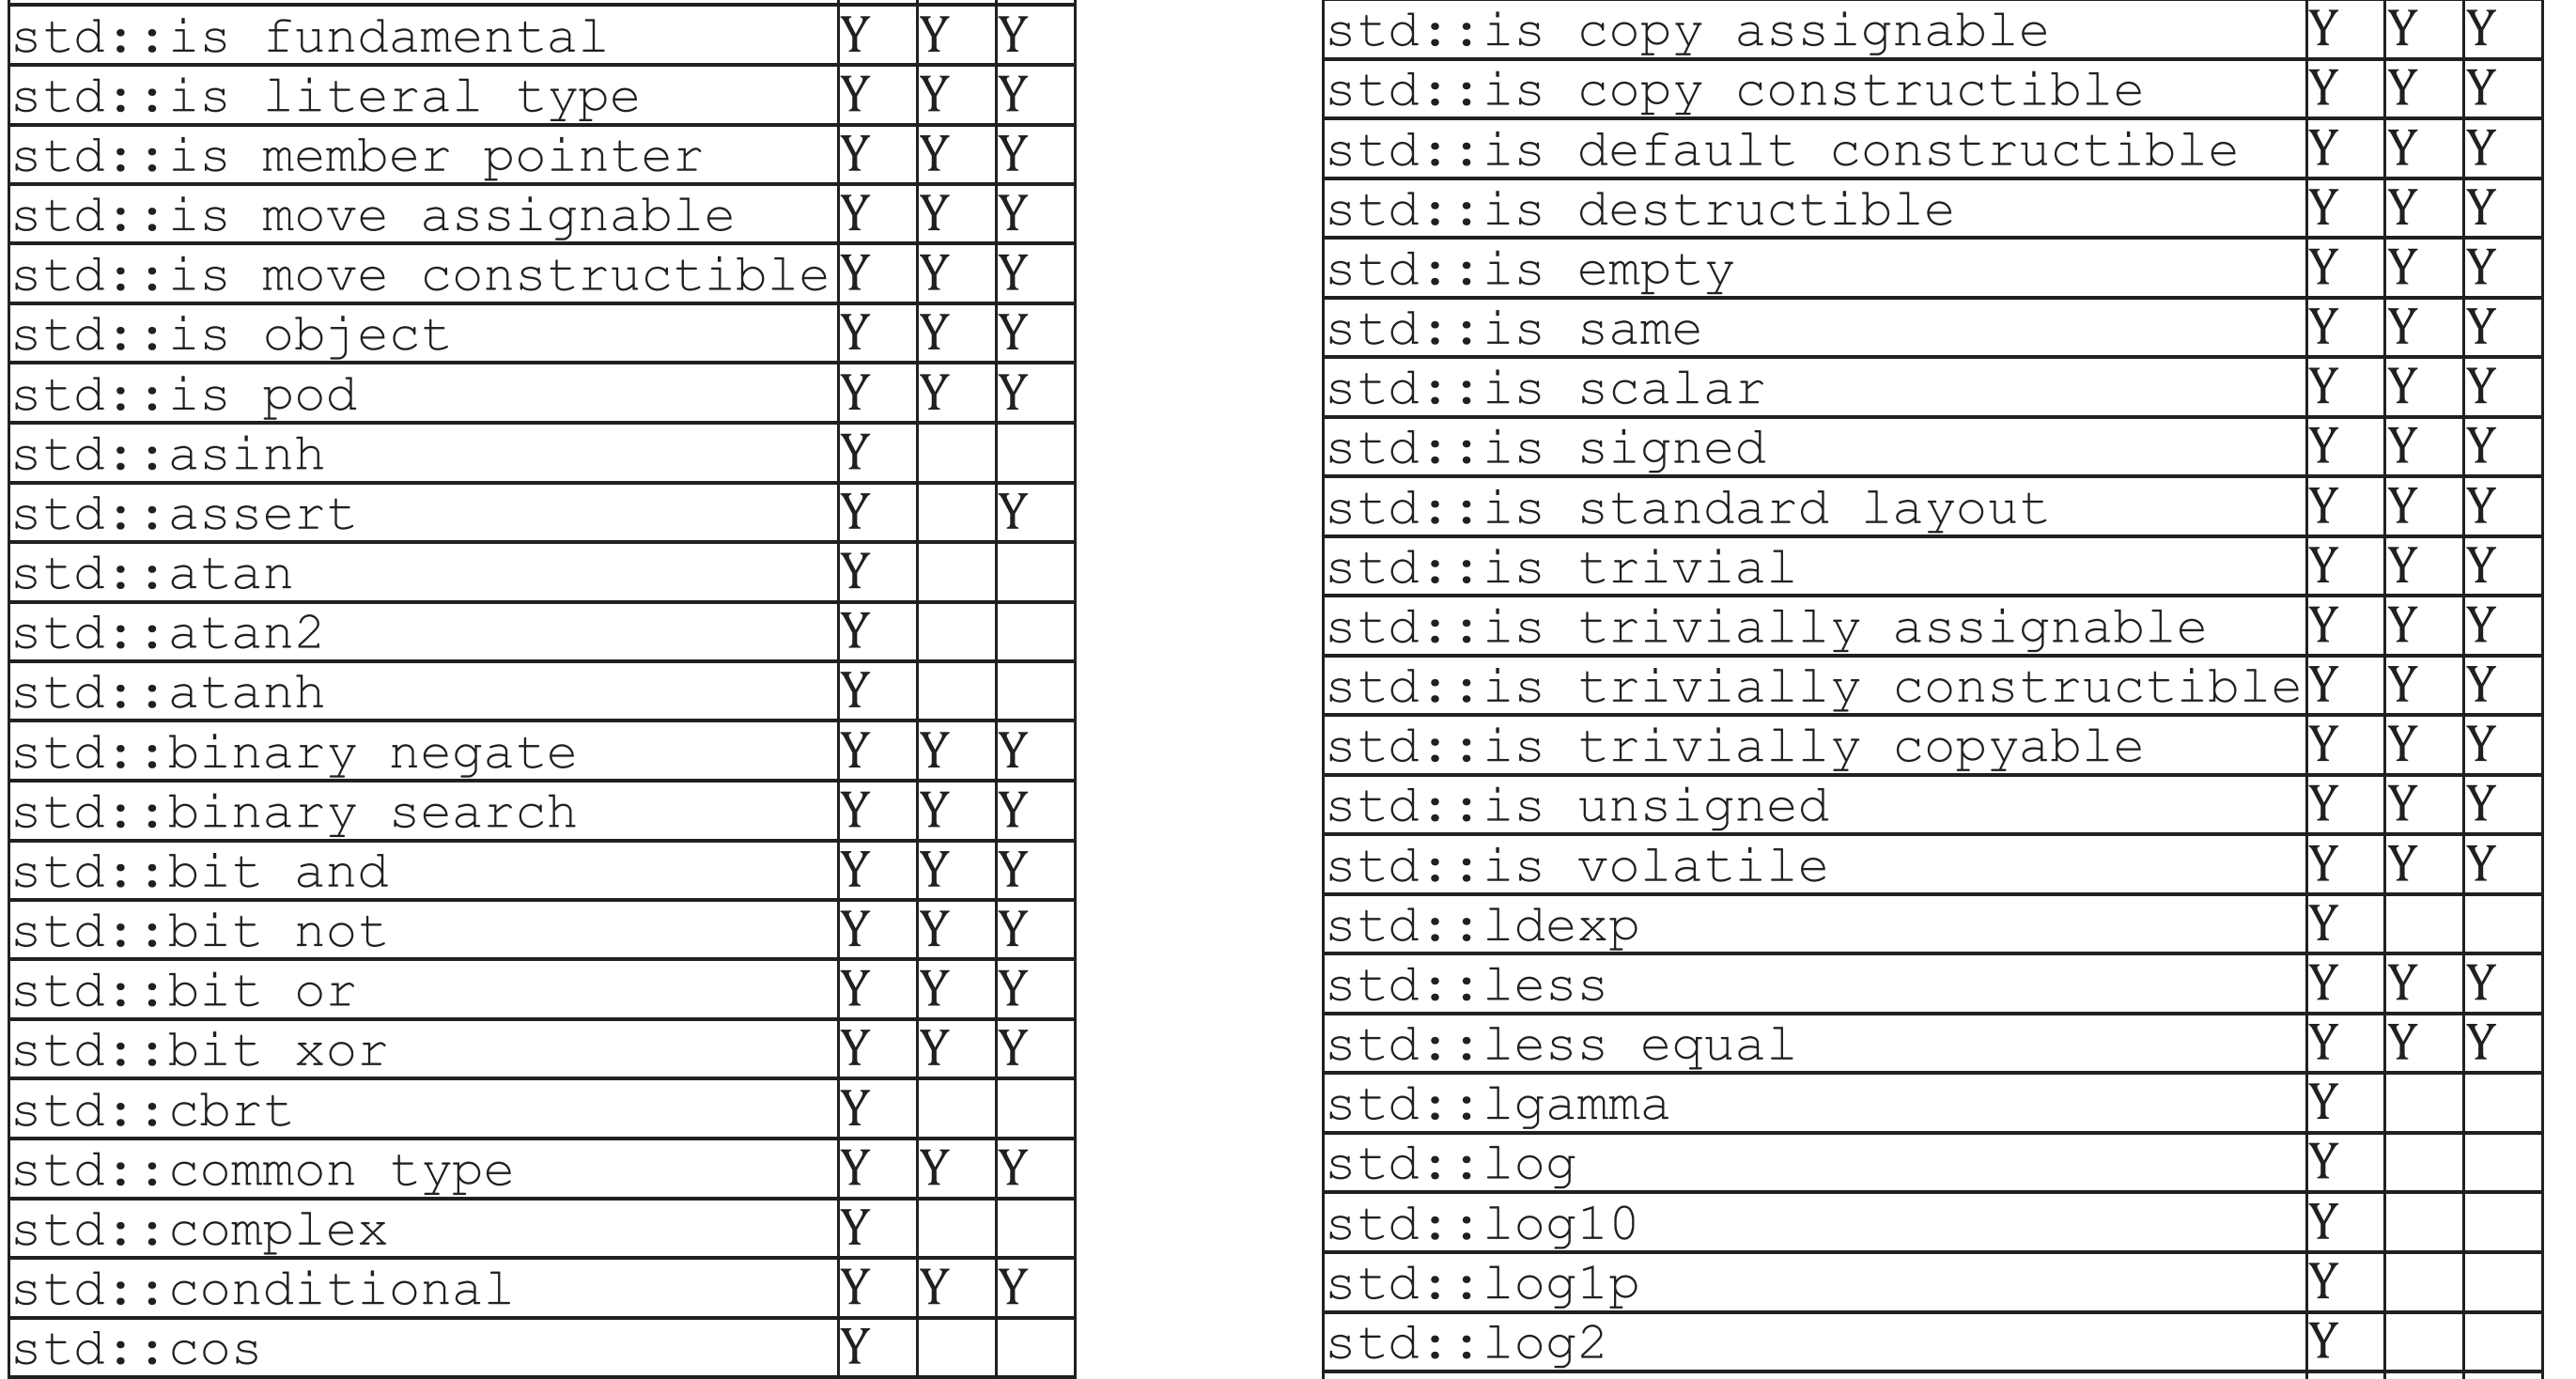
\includegraphics[width=1.0\textwidth]{content/chapter-18/images/8}
	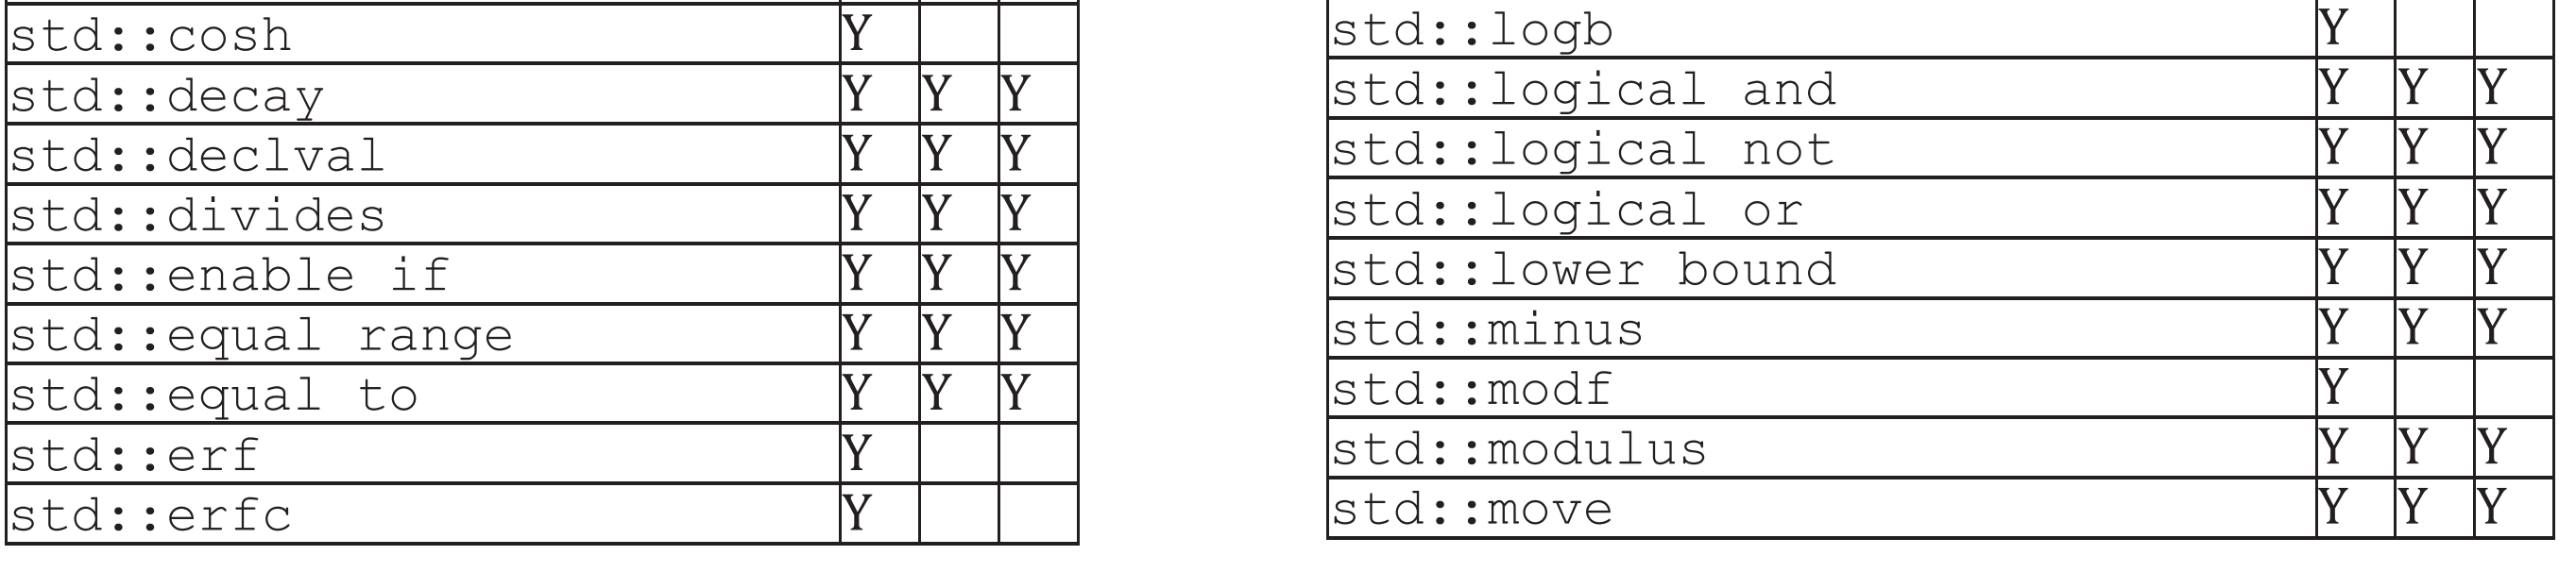
\includegraphics[width=1.0\textwidth]{content/chapter-18/images/9}
	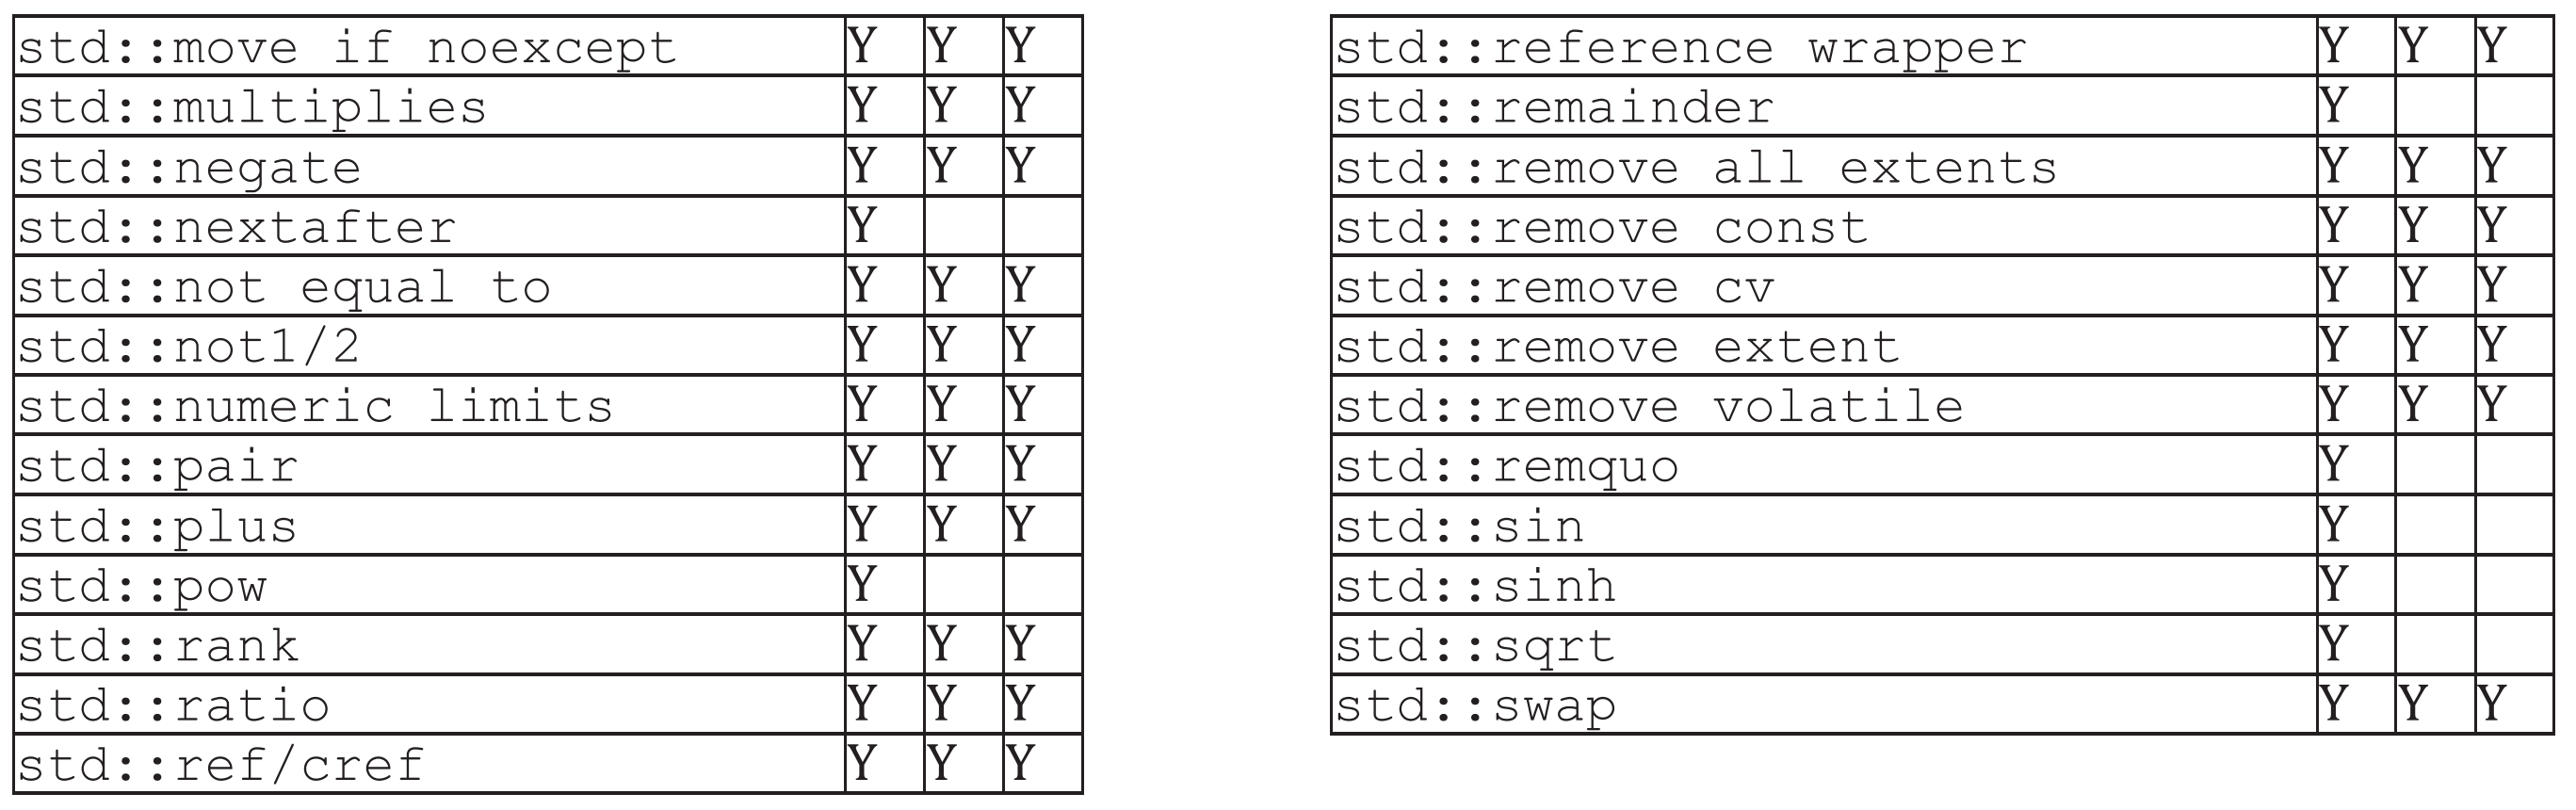
\includegraphics[width=1.0\textwidth]{content/chapter-18/images/10}
\end{center}

The tested standard C++ APIs are supported in libstdc++ (GNU) with gcc 7.4.0 and libc++ (LLVM) with clang 10.0 and MSVC Standard C++ Library with Microsoft Visual Studio 2017 for the host CPU as well.\par

On Linux, GNU libstdc++ is the default C++ standard library for the DPC++ compiler, so no compilation or linking option is required. If we want to use libc++, use the compile options -stdlib=libc++ -nostdinc++ to leverage libc++ and to not include C++ std headers from the system. The DPC++ compiler has been verified using libc++ in DPC++ kernels on Linux, but the DPC++ runtime needs to be rebuilt with libc++ instead of libstdc++. Details are in https://intel.github.io/llvmdocs/GetStartedGuide.html\#build-dpc-toolchain-with-libc-library. Because of these extra steps, libc++ is not the recommended C++ standard library for us to use in general.\par

On FreeBSD, libc++ is the default standard library, and the -stdlib=libc++ option is not required. More details are in https://libcxx.llvm.org/docs/UsingLibcxx.html. On Windows, only the MSVC C++ library can be used.\par

\begin{tcolorbox}[colback=red!5!white,colframe=red!75!black]
To achieve cross-architecture portability, if a std function is not marked with “Y” in Figure 18-8, we need to keep portability in mind when we write device functions!
\end{tcolorbox}

\hspace*{\fill} \par %插入空行
\textbf{DPC++ Parallel STL}

Parallel STL is an implementation of the C++ standard library algorithms with support for execution policies, as specified in the ISO/IEC 14882:2017 standard, commonly called C++17. The existing implementation also supports the unsequenced execution policy specified in Parallelism TS version 2 and proposed for the next version of the C++ standard in the C++ working group paper P1001R1.\par

When using algorithms and execution policies, specify the namespace std::execution if there is no vendor-specific implementation of the C++17 standard library or pstl::execution otherwise.\par

For any of the implemented algorithms, we can pass one of the values seq, unseq, par, or par\_unseq as the first parameter in a call to the algorithm to specify the desired execution policy. The policies have the following meanings:\par

\begin{table}[]
	\begin{tabular}{|l|l|}
		\hline
		Execution Policy & Meaning                                                                                                                                            \\ \hline
		seq              & Sequential execution.                                                                                                                              \\ \hline
		unseq            & \begin{tabular}[c]{@{}l@{}}Unsequenced SIMD execution. This policy requires that\\ all functions proided are safe to execute in SIMD.\end{tabular} \\ \hline
		par              & Parallel execution by multiple threads.                                                                                                            \\ \hline
		par\_unseq       & Combined effect of unseq an par                                                                                                                    \\ \hline
	\end{tabular}
\end{table}

Parallel STL for DPC++ is extended with support for DPC++ devices using special execution policies. The DPC++ execution policy specifies where and how a Parallel STL algorithm runs. It inherits a standard C++ execution policy, encapsulates a SYCL device or queue, and allows us to set an optional kernel name. DPC++ execution policies can be used with all standard C++ algorithms that support execution policies according to the C++17 standard.\par

\hspace*{\fill} \par %插入空行
\textbf{DPC++ Execution Policy}

Currently, only the parallel unsequenced policy (par\_unseq) is supported by the DPC++ library. In order to use the DPC++ execution policy, there are three steps:\par

\begin{enumerate}
	\item Add \#include <dpstd/execution> into our code.
	\item Create a policy object by providing a standard 
	policy type, a class type for a unique kernel name 
	as a template argument (optional), and one of the 
	following constructor arguments:
	\begin{itemize}
		\item A SYCL queue
		\item A SYCL device
		\item A SYCL device selector
		\item An existing policy object with a different kernel 		name
	\end{itemize}
	\item Pass the created policy object to a Parallel STL algorithm.
\end{enumerate}

A dpstd::execution::default\_policy object is a predefined device\_policy created with a default kernel name and default queue. This can be used to create custom policy objects or passed directly when invoking an algorithm if the default choices are sufficient.\par

Figure 18-9 shows examples that assume use of the using namespace dpstd::execution; directive when referring to policy classes and functions.\par

\hspace*{\fill} \par %插入空行
Figure 18-9. Creating execution policies
\begin{lstlisting}[caption={}]
auto policy_b = 
	device_policy<parallel_unsequenced_policy, class PolicyB> 
		{sycl::device{sycl::gpu_selector{}}};
std::for_each(policy_b, …);

auto policy_c = 
	device_policy<parallel_unsequenced_policy, class PolicyС> 
		{sycl::default_selector{}};
std::for_each(policy_c, …);

auto policy_d = make_device_policy<class PolicyD>(default_policy);
std::for_each(policy_d, …);

auto policy_e = make_device_policy<class PolicyE>(sycl::queue{});
std::for_each(policy_e, …);
\end{lstlisting}

\hspace*{\fill} \par %插入空行
\textbf{FPGA Execution Policy}

The fpga\_device\_policy class is a DPC++ policy tailored to achieve better performance of parallel algorithms on FPGA hardware devices. Use the policy when running the application on FPGA hardware or an FPGA emulation device:\par

\begin{enumerate}
	\item Define the \_PSTL\_FPGA\_DEVICE macro to run on FPGA devices and additionally \_PSTL\_FPGA\_EMU to run on an FPGA emulation device.
	\item Add \#include <dpstd/execution> to our code.
	\item Create a policy object by providing a class type for a unique kernel name and an unroll factor (see Chapter 17) as template arguments (both optional) and one of the following constructor arguments:
	\begin{itemize}
		\item A SYCL queue constructed for the FPGA selector (the behavior is undefined with any other device type)
		\item An existing FPGA policy object with a different kernel name and/or unroll factor
	\end{itemize}
	\item Pass the created policy object to a Parallel STL algorithm.
\end{enumerate}

The default constructor of fpga\_device\_policy creates an object with a SYCL queue constructed for fpga\_selector, or for fpga\_emulator\_selector if \_PSTL\_FPGA\_EMU is defined.\par

dpstd::execution::fpga\_policy is a predefined object of the fpga\_device\_policy class created with a default kernel name and default unroll factor. Use it to create customized policy objects or pass it directly when invoking an algorithm.\par

Code in Figure 18-10 assumes using namespace dpstd::execution; for policies and using namespace sycl; for queues and device selectors.\par

Specifying an unroll factor for a policy enables loop unrolling in the implementation of algorithms. The default value is 1. To find out how to choose a better value, see Chapter 17.\par

\hspace*{\fill} \par %插入空行
Figure 18-10. Using FPGA policy
\begin{lstlisting}[caption={}]
auto fpga_policy_a = fpga_device_policy<class FPGAPolicyA>{};

auto fpga_policy_b = make_fpga_policy(queue{intel::fpga_selector{}});

constexpr auto unroll_factor = 8;
auto fpga_policy_c = 
make_fpga_policy<class FPGAPolicyC, unroll_factor>(fpga_policy);
\end{lstlisting}

\hspace*{\fill} \par %插入空行
\textbf{Using DPC++ Parallel STL}

In order to use the DPC++ Parallel STL, we need to include Parallel STL header files by adding a subset of the following set of lines. These lines are dependent on the algorithms we intend to use:\par

\begin{itemize}
	\item \#include <dpstd/algorithm>
	\item \#include <dpstd/numeric>
	\item \#include <dpstd/memory>
\end{itemize}

dpstd::begin and dpstd::end are special helper functions that allow us to pass SYCL buffers to Parallel STL algorithms. These functions accept a SYCL buffer and return an object of an unspecified type that satisfies the following requirements:\par

\begin{itemize}
	\item Is CopyConstructible, CopyAssignable, and 	comparable with operators == and !=.
	\item The following expressions are valid: a + n, a – n, and a – b, where a and b are objects of the type and n is an integer value.
	\item Has a get\_buffer method with no arguments. The method returns the SYCL buffer passed to dpstd::begin and dpstd::end functions.
\end{itemize}

To use these helper functions, add \#include <dpstd/iterators> to our code. See the code in Figures 18-11 and 18-12 using the std::fill function as examples that use the begin/end helpers.\par

\hspace*{\fill} \par %插入空行
Figure 18-11. Using std::fill
\begin{lstlisting}[caption={}]
#include <dpstd/execution>
#include <dpstd/algorithm>
#include <dpstd/iterators>

sycl::queue Q;
sycl::buffer<int> buf { 1000 };

auto buf_begin = dpstd::begin(buf);
auto buf_end = dpstd::end(buf);

auto policy = dpstd::execution::make_device_policy<class fill>( Q );
std::fill(policy, buf_begin, buf_end, 42);
// each element of vec equals to 42
\end{lstlisting}

\begin{tcolorbox}[colback=blue!5!white,colframe=blue!75!black, title=REDUCE DATA COPYING BETWEEN THE HOST AND DEVICE]
Parallel STL algorithms can be called with ordinary (host-side) iterators, as seen in the code example in Figure 18-11.\\

In this case, a temporary SYCL buffer is created, and the data is copied to this buffer. After processing of the temporary buffer on a device is complete, the data is copied back to the host. Working directly with existing SYCL buffers, where possible, is recommended to reduce data movement between the host and device and any unnecessary overhead of buffer creations and destructions.
\end{tcolorbox}

\hspace*{\fill} \par %插入空行
Figure 18-12. Using std::fill with default policy
\begin{lstlisting}[caption={}]
#include <dpstd/execution>
#include <dpstd/algorithm>

std::vector<int> v( 1000000 );
std::fill(dpstd::execution::default_policy, v.begin(), v.end(), 42);
// each element of vec equals to 42
\end{lstlisting}

Figure 18-13 shows an example which performs a binary search of the input sequence for each of the values in the search sequence provided. As the result of a search for the ith element of the search sequence, a Boolean value indicating whether the search value was found in the input sequence is assigned to the ith element of the result sequence. The algorithm returns an iterator that points to one past the last element of the result sequence that was assigned a result. The algorithm assumes that the input sequence has been sorted by the comparator provided. If no comparator is provided, then a function object that uses operator< to compare the elements will be used.\par

The complexity of the preceding description highlights that we should leverage library functions where possible, instead of writing our own implementations of similar algorithms which may take significant debugging and tuning time. Authors of the libraries that we can take advantage of are often experts in the internals of the device architectures to which they are coding, and may have access to information that we do not, so we should always leverage optimized libraries when they are available.\par

The code example shown in Figure 18-13 demonstrates the three typical steps when using a DPC++ Parallel STL algorithm:\par

\begin{itemize}
	\item Create DPC++ iterators.
	\item Create a named policy from an existing policy.
	\item Invoke the parallel algorithm
\end{itemize}

The example in Figure 18-13 uses the dpstd::binary\_search algorithm to perform binary search on a CPU, GPU, or FPGA, based on our device selection.\par

\hspace*{\fill} \par %插入空行
Figure 18-13. Using binary\_search
\begin{lstlisting}[caption={}]
#include <dpstd/execution>
#include <dpstd/algorithm>
#include <dpstd/iterator>

buffer<uint64_t, 1> kB{ range<1>(10) };
buffer<uint64_t, 1> vB{ range<1>(5) };
buffer<uint64_t, 1> rB{ range<1>(5) };

accessor k{kB};
accessor v{vB};

// create dpc++ iterators
auto k_beg = dpstd::begin(kB);
auto k_end = dpstd::end(kB);
auto v_beg = dpstd::begin(vB);
auto v_end = dpstd::end(vB);
auto r_beg = dpstd::begin(rB);

// create named policy from existing one
auto policy = dpstd::execution::make_device_policy<class bSearch>
	(dpstd::execution::default_policy);

// call algorithm
dpstd::binary_search(policy, k_beg, k_end, v_beg, v_end, r_beg);

// check data
accessor r{rB};
if ((r[0] == false) && (r[1] == true) && 
(r[2] == false) && (r[3] == true) && (r[4] == true)) {
	std::cout << "Passed.\nRun on "
	<< policy.queue().get_device().get_info<info::device::name>()
	<< "\n";
} else
	std::cout << "failed: values do not match.\n";
\end{lstlisting}

\hspace*{\fill} \par %插入空行
\textbf{Using Parallel STL with USM}

The following examples describe two ways to use the Parallel STL algorithms in combination with USM:\par

\begin{itemize}
	\item Through USM pointers
	\item Through USM allocators
\end{itemize}

If we have a USM allocation, we can pass the pointers to the start and (one past the) end of the allocation to a parallel algorithm. It is important to be sure that the execution policy and the allocation itself were created for the same queue or context, to avoid undefined behavior at runtime.\par

If the same allocation is to be processed by several algorithms, either use an in-order queue or explicitly wait for completion of each algorithm before using the same allocation in the next one (this is typical operation ordering when using USM). Also wait for completion before accessing the data on the host, as shown in Figure 18-14.\par

Alternatively, we can use std::vector with a USM allocator as shown in Figure 18-15.\par

\hspace*{\fill} \par %插入空行
Figure 18-14. Using Parallel STL with a USM pointer
\begin{lstlisting}[caption={}]
#include <dpstd/execution>
#include <dpstd/algorithm>

sycl::queue q;
const int n = 10;
int* d_head = static_cast<int*>(
	sycl::malloc_device(n * sizeof(int),
						q.get_device(), 
						q.get_context()));
						
std::fill(dpstd::execution::make_device_policy(q),
		  d_head, d_head + n, 78);
q.wait();

sycl::free(d_head, q.get_context());
\end{lstlisting}

\hspace*{\fill} \par %插入空行
Figure 18-15. Using Parallel STL with a USM allocator
\begin{lstlisting}[caption={}]
#include <dpstd/execution>
#include <dpstd/algorithm>

sycl::queue Q;
const int n = 10;
sycl::usm_allocator<int, sycl::usm::alloc::shared> 
						 alloc(Q.get_context(), Q.get_device());
std::vector<int, decltype(alloc)> vec(n, alloc);

std::fill(dpstd::execution::make_device_policy(Q), 
							vec.begin(), vec.end(), 78);
Q.wait();
\end{lstlisting}

\hspace*{\fill} \par %插入空行
\textbf{Error Handling with DPC++ Execution Policies}

As detailed in Chapter 5, the DPC++ error handling model supports two types of errors. With synchronous errors, the runtime throws exceptions, while asynchronous errors are only processed in a user-supplied error handler at specified times during program execution.\par

For Parallel STL algorithms executed with DPC++ policies, handling of all errors, synchronous or asynchronous, is a responsibility of the caller. Specifically\par

\begin{itemize}
	\item No exceptions are thrown explicitly by algorithms.
	\item Exceptions thrown by the runtime on the host CPU, including DPC++ synchronous exceptions, are passed through to the caller.
	\item DPC++ asynchronous errors are not handled by the Parallel STL, so must be handled (if any handling is desired) by the calling application.
\end{itemize}

To process DPC++ asynchronous errors, the queue associated with a DPC++ policy must be created with an error handler object. The predefined policy objects (default\_policy and others) have no error handlers, so we should create our own policies if we need to process asynchronous errors.\par

































